\begin{center}
\textbf{\Large Треугольник Паскаля}\\
%\textit{Профи}\\
\textit{11.07.16}
\end{center}

\epigraph{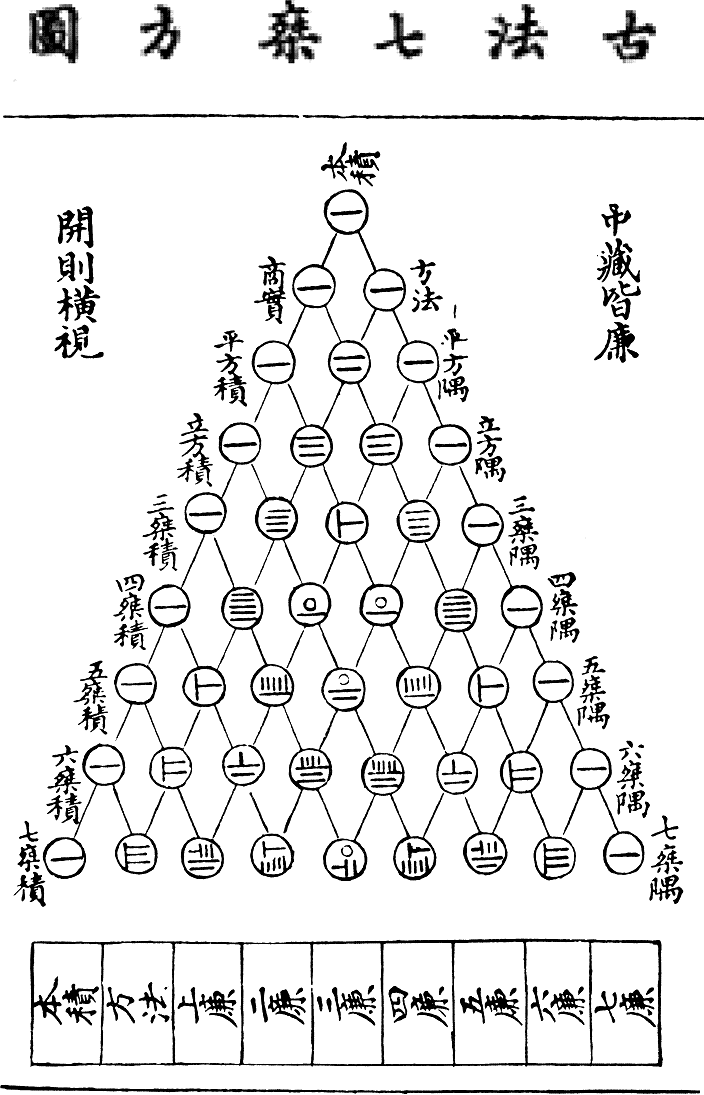
\includegraphics[width=.8\textwidth]{Yanghui_triangle}}{Треугольник Яна Хуэя, 1303}

\textbf{Задача.} Черепашка Пося находится в нижнем левом углу таблицы $(n+1)\times (m+1)$. За один ход Пося может переползти на одну клетку вверх или на одну клетку вправо. Сколько существует способов добраться до верхнего правого угла таблицы?

\begin{problems}
 
\item а) Пронумеруем строки от 1 до $(n+1)$, столбцы от 1 до $(m+1)$. Пусть черепашка начинает движение из клетки $(1, 1)$. Докажите, что количество способов добраться до клетки $(x, y)$ равно количеству способов добраться до клетки $(x-1, y)$ плюс количество способов добраться до клетки $(x, y-1)$.\\
б) Решите задачу про черепашку для $n=m=5$.

\item а) Мы выдрессировали черепашку. Теперь мы ей говорим, когда ползти вверх, а когда ползти вправо. Чтобы запомнить как именно черепашка ползёт, мы записываем очередность наших команд. Сколько вариантов записей могло получиться, если черепашка в итоге оказалась в клетке $(n+1, 2)$?\\
б) Решите задачу про черепашку Посю.

\item Посмотрите, куда черепашка может доползти за $n$ шагов и докажите тождество:
$$C_n^0+C_n^1+\cdots+C_n^n=2^n.$$

\item Пока мальчик Вова командует черепашкой, мальчик Лёня начал раскрывать скобки выражения:
$$(a+b)^n=(a+b)(a+b)\cdots (a+b).$$
Но получилось так, что когда Лёня умножал слагаемое на $a$, то Вова говорил черепашке ползти вверх, а если Лёня умножал слагаемое на $b$, то Вова говорил черепашке ползти вправо. В конце концов Лёня привел подобные слагаемые. Выразите получившиеся коэффициенты. 
\end{problems}

Запишем в каждую клетку таблицы число, равное количеству способов добраться до этой клетки. Повернем нашу таблицу так, чтобы все числа, отвечающие за одинаковое количество ходов, были на одном уровне. Результат называется \textbf{треугольником Паскаля}.

На краях этого треугольника стоят единицы, а каждое число внутри является суммой двух, стоящих над ним. $k$-е число $n$-й строки треугольника Паскаля равно $C_n^k$ (строки нумеруются сверху вниз, начиная с нуля, а числа в строках нумеруются слева направо, также начиная с нуля).

\begin{figure}[h!]
\center{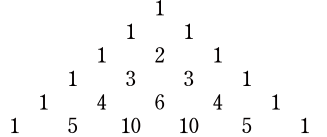
\includegraphics[scale=0.5]{pasc.png}}
\end{figure}

Коэффициенты разложения из 4 задачи называются \textbf{бином Ньютона.}
% \newpage
\begin{problems}
\item Вычислите выражение $C_n^0-C_n^1+C_n^2-\cdots\pm C_n^n$\\
а) используя треугольник Паскаля;\\
б) используя бином Ньютона.

\item У Тома Сойера есть забор из $2n$ досок и белая краска. Сколькими способами он может покрасить в этом заборе четное число досок?

\item Чему равно $C_k^k+C_{k+1}^k+\cdots+C_n^k$?

\item а) Для каждой из первых 4 строчек треугольника Паскаля сложите квадраты стоящих в ней чисел и найдите полученное число в треугольнике Паскаля. Запишите полученное тождество.\\
б) Докажите это тождество.
\end{problems}

\textbf{Числа Фибоначчи}~--- последовательность чисел:
$$1, \;1, \;2, \;3, \;5, \;8, \;13, \;21, \;34, \;55, \;89,\dots,$$
удовлетворяющая условию $F_0=1, F_1=1, F_{n+2}=F_{n+1}+F_n.$

\begin{problems}
\item Используя треугольник Паскаля докажите тождество: $$F_n=C_n^0+C_{n-1}^1+C_{n-2}^2+\cdots.$$
\end{problems}
